% !TeX encoding = UTF-8
% !TeX root = ../main.tex

%% ------------------------------------------------------------------------
%% Copyright (C) 2021-2023 SJTUG
%% 
%% SJTUBeamer Example Document by SJTUG
%% 
%% SJTUBeamer Example Document is licensed under a
%% Creative Commons Attribution-NonCommercial-ShareAlike 4.0 International License.
%% 
%% You should have received a copy of the license along with this
%% work. If not, see <http://creativecommons.org/licenses/by-nc-sa/4.0/>.
%% -----------------------------------------------------------------------

\section{动态规划分题型讲解}
\subsection{基本理论概括}

\begin{frame}[fragile]
  \frametitle{一些简单的思想概括}
  \begin{itemize}
    \item 记忆化搜索与\lstinline{@cache}装饰器

          \begin{itemize}
            \item 记忆化搜索相对于递推来说,实现逻辑更加简单,但是有时候只有写成递推形式才能结合数据结构优化时间复杂度
            \item 但是大部分时候记忆化搜索是动态规划题目的神兵利器
          \end{itemize}

    \item \textbf{动态规划类型划分}:动态规划题型多样,每一种都有相对应的解法

          \begin{itemize}
            \item 网格图\textsc{DP}
            \item 背包\textsc{DP}
            \item 线性\textsc{DP}
            \item 状态机\textsc{DP}
            \item 划分型\textsc{DP}
            \item 其他线性\textsc{DP}
            \item 区间\textsc{DP}
            \item 状态压缩\textsc{DP}
            \item 数据结构优化\textsc{DP}
            \item 树形\textsc{DP}
          \end{itemize}
  \end{itemize}
\end{frame}

\subsubsection{背包\textsc{DP}}

\begin{frame}{0-1背包的思想和公式}
  \begin{alertblock}{核心思想是“选与不选”两个问题}
    \begin{equation*}
      dp(i,target)=\max(dp(i-1,target),dp(i-1,target-weight[i])+value[i])
    \end{equation*}
  \end{alertblock}
  \begin{itemize}
    \item \textbf{基本问题}:有一系列重量为$weight$,价值为$value$的物品,背包容量为$target$,求最大价值
    \item  用$dp(i,target)$表示:\textsc{到第$i$个物品,背包容量为$target$时的最大价值}
           \begin{itemize}
            \item 不选当前物品:$dp(i, target)=dp(i-1,target)$
            \item 选当前物品:$dp(i, target)=dp(i-1,target-weight[i])+value[i]$
           \end{itemize}
    \item  合起来就是$dp(i,target)=\max(dp(i-1,target),dp(i-1,target-weight[i])+value[i])$
    \item 在自己实现的时候最好用记忆化搜索和递推两种方法都实现一遍    
  \end{itemize}
\end{frame}


\begin{frame}[fragile]          % 注意添加 fragile 标记
  \frametitle{\textsc{举个栗子:416. 分割等和子集\link{https://leetcode.cn/problems/partition-equal-subset-sum/}}}
  % 代码块参数:语言,标题
  % 请减少代码初始的缩进
  \begin{itemize}
    \item 定义$dp(i,target)$为从0到前$i$个物品中选,\textbf{是否}能选出和\textbf{恰好为$target$}(\lstinline{return True/False})
    \item 对于第$i$个物品,要么选要么不选
        \begin{itemize}
          \item 如果不选:$dp(i,target)=dp(i-1,target)$
          \item 如果选了,那么$dp(i,target)=dp(i-1,target-nums[i])$
        \end{itemize}
    \item 合起来就是$dp(i,target)=dp(i-1,target) | dp(i-1,target-nums[i])$
    \item 想ac一道dp题,那么肯定是需要考虑好边界条件的。递推的入口是哪里呢?  
         \begin{itemize}
          \item 没有物品可以选,也就是$i<0$或者$i==n$。此时$target==0$的时候才能\lstinline{return True},不然没东西选必然凑不出一些物品,让这些物品的和为$target$。
          \item 所以可以写成:\lstinline{if i < 0: return True if target == 0 else False},或者\lstinline{if i == n: return True if target == 0 else False},看你喜欢哪种了
         \end{itemize}
  \end{itemize}
\end{frame}


\begin{frame}[fragile]          % 注意添加 fragile 标记
  \frametitle{说了这么多看看代码怎么写吧!我们新上手建议采用两种方式都实现一下}
  % 代码块参数:语言,标题
  % 请减少代码初始的缩进
  \begin{codeblock}[language=python]{记忆化搜索版本的代码}
class Solution:
def canPartition(self, nums: List[int]) -> bool:
  @cache
  def dfs(i: int, target: int) -> bool:
      if i < 0:
          return True if target == 0 else False
      ans = dfs(i - 1, target)
      if target >= nums[i]:
          ans = ans | dfs(i - 1, target - nums[i])
      return ans
  s = sum(nums)

  \end{codeblock}
\end{frame}

\begin{frame}[fragile]          % 注意添加 fragile 标记
  \frametitle{}
  % 代码块参数:语言,标题
  % 请减少代码初始的缩进
  \begin{codeblock}[language=python]{}
  if s & 1 == 1:
  return False

  ans = dfs(len(nums) - 1, s // 2)
  dfs.cache_clear()
  return ans

  \end{codeblock}
  或者这样
  \begin{codeblock}[language=python]{}
class Solution:
  def canPartition(self, nums: List[int]) -> bool:
    @cache
    def dfs(i: int, target: int) -> bool:
        if i == len(nums):
            return True if target == 0 else False
        ans = dfs(i + 1, target)
        if target >= nums[i]:
            ans = ans | dfs(i + 1, target - nums[i])
        return ans
    \end{codeblock}
\end{frame}

\begin{frame}[fragile]          % 注意添加 fragile 标记
  \frametitle{}
  % 代码块参数:语言,标题
  % 请减少代码初始的缩进
  \begin{codeblock}[language=python]{}
    s = sum(nums)
    if s & 1 == 1:
        return False
    
    ans = dfs(0, s // 2)
    dfs.cache_clear()
    return ans

  \end{codeblock}
  1:1翻译成递推
  \begin{codeblock}[language=python]{}
class Solution:
    def canPartition(self, nums: List[int]) -> bool:
        s = sum(nums)
        if s % 2 == 1:
            return False
        s //= 2
        n = len(nums)
        dp = [[False] * (s + 1) for _ in range(n + 1)]
        dp[0][0] = True
 
    \end{codeblock}
\end{frame}


\begin{frame}[fragile]          % 注意添加 fragile 标记
  \frametitle{}
  % 代码块参数:语言,标题
  % 请减少代码初始的缩进
  \begin{codeblock}[language=python]{}
    for i, num in enumerate(nums):
    for target in range(s + 1):
        dp[i + 1][target] = target >= num and dp[i][target - num] or dp[i][target]
    return dp[n][s]

  \end{codeblock}
\end{frame}



\begin{frame}[fragile]          % 注意添加 fragile 标记
  \frametitle{\textsc{2915. 和为目标值的最长子序列的长度}\link{https://leetcode.cn/problems/length-of-the-longest-subsequence-that-sums-to-target}}
  % 代码块参数:语言,标题
  % 请减少代码初始的缩进
  \begin{alertblock}{核心思想依然是“选与不选”}
    \begin{equation*}
      dp(i,target)=\max(dp(i-1,target),dp(i-1,target-nums[i])+1)
    \end{equation*}
  \end{alertblock}
  \begin{itemize}
    \item $dp(i,target)=dp(i-1,target)$老样子,代表不选
    \item $dp(i,target)=dp(i-1,target - nums[i]) + 1$。你既然不选,那么\textbf{长度不变}依然继承$dp(i-1,target)$;如果你选了那么长度肯定++咯
    \item 合起来,那么$dp(i,target)=\max(dp(i-1,target),dp(i-1,target-nums[i])+1)$
    \item 注意边界条件。如果没有东西可以选,我们还希望和为$target$,那么只有$target=0$的时候才有意义,让长度为0。否则不可能做到,长度必为$-\infty$
  \end{itemize}
\end{frame}



\begin{frame}[fragile]          % 注意添加 fragile 标记
  
  % 代码块参数:语言,标题
  % 请减少代码初始的缩进
  \begin{codeblock}[language=python]{记忆化搜索版本的代码}
class Solution:
    def lengthOfLongestSubsequence(self, nums: List[int], target: int) -> int:
        @cache
        def dfs(i: int, target: int) -> int:
            if i < 0:
                return 0 if target == 0 else -inf
            ans = dfs(i - 1, target)
            if target >= nums[i]:
                ans = max(ans, dfs(i - 1, target - nums[i]) + 1)
            return ans
        ans = dfs(len(nums) - 1, target)
        dfs.cache_clear()
        return ans if ans != -inf else -1
  \end{codeblock}
\end{frame}


\begin{frame}[fragile]          % 注意添加 fragile 标记
  \frametitle{1:1翻译成递推}
  % 代码块参数:语言,标题
  % 请减少代码初始的缩进
  \begin{codeblock}[language=python]{}
class Solution:
    def lengthOfLongestSubsequence(self, nums: List[int], target: int) -> int:
        n = len(nums)
        dp = [[-inf] * (target + 1) for _ in range(n + 1)]
        dp[0][0] = 0
        for i, num in enumerate(nums):
            for j in range(target + 1):
                dp[i + 1][j] = dp[i][j]
                if j >= nums[i]:
                    dp[i + 1][j] = max(dp[i][j], dp[i][j - nums[i]] + 1)
        ans = dp[n][target]
        return ans if ans != -inf else -1
  \end{codeblock}
\end{frame}


\begin{frame}[fragile]          % 注意添加 fragile 标记
  \frametitle{因为$dp[i+1][j]$是从$dp[i][j]$推导出来的,我们优化掉$i$这个维度}
  % 代码块参数:语言,标题
  % 请减少代码初始的缩进
  \begin{codeblock}[language=python]{在有些题可以结合数据结构比如线段树来优化$DP$}
class Solution:
    def lengthOfLongestSubsequence(self, nums: List[int], target: int) -> int:
        n = len(nums)
        dp = [0] + [-inf] * target
        for num in nums:
            for j in range(target, num - 1, -1):
                if dp[j - num] + 1 > dp[j]:
                    dp[j] = dp[j - num] + 1
        ans = dp[-1]
        return ans if ans != -inf else -1
  \end{codeblock}
\end{frame}


\begin{frame}[fragile]          % 注意添加 fragile 标记
  \frametitle{\textsc{494. 目标和}\link{https://leetcode.cn/problems/target-sum}}
  % 代码块参数:语言,标题
  % 请减少代码初始的缩进
  \begin{alertblock}{怎么转换成“选与不选”经典问题呢?}
    \begin{equation*}
      dp(i,target)=dp(i-1,target)+dp(i-1,target-nums[i])
    \end{equation*}
  \end{alertblock}
  \begin{itemize}
    \item 如果$nums[0],nums[1],\dots,nums[-1]$这些数中,有一些数前面的符号是$+$,另一些数前面的符号一定是$-$。
    \item 我们记$+$的这些数,和为$p$,这些带减号的,和为$q$。比如示例1:$nums=[1,1,1,1,1],target=3$,一种方案是$-1+1+1+1+1=3$
    \item 那么,我们的$q=1$,$p=4$。那么$p+q=sum(nums)$,$p-q=target$。那么我们就有了$p=(sum(nums)+target)/2$。如果我们没有$nums$可选,$p=0$的时候什么都没有也是一个方案,$dp(0,0)=1$
    \item 那么我们的问题就变成了:在$nums$中选出一些数,使得他们的和为$p$。方案有多少呢?这就是一个经典的对于$nums[i]$,\textbf{选与不选}的\textbf{背包}问题了。
    \item 对于每一个$nums[i]$,我们有选与不选两种选择。也就是上面公式的两项了
  \end{itemize}
\end{frame}



\begin{frame}[fragile]          % 注意添加 fragile 标记
  
  % 代码块参数:语言,标题
  % 请减少代码初始的缩进
  \begin{codeblock}[language=python]{记忆化搜索版本的代码}
class Solution:
    def findTargetSumWays(self, nums: List[int], target: int) -> int:
        s = sum(nums)
        if (s + target) < 0 or (s + target) % 2:
            return 0
        target = (s + target) // 2
        @cache
        def dfs(i: int, target: int) -> int:
            if i < 0:
                return 1 if target == 0 else 0
            return dfs(i - 1, target) + dfs(i - 1, target - nums[i])
        return dfs(len(nums) - 1, target)
  \end{codeblock}
\end{frame}


\begin{frame}[fragile]          % 注意添加 fragile 标记
  \frametitle{$dp[i][j]=dp[i-1][j]+dp[i-1][j-nums[i]]$}
  % 代码块参数:语言,标题
  % 请减少代码初始的缩进
  \begin{codeblock}[language=python]{1:1翻译成优化一个维度的递推}
class Solution:
    def findTargetSumWays(self, nums: List[int], target: int) -> int:
        s = sum(nums)
        if (s + target) < 0 or (s + target) % 2:
            return 0
        target = (s + target) // 2
        dp = [1] + [0] * target
        for num in nums:
            for j in range(target, num - 1, -1):
                dp[j] += dp[j - num]
        return dp[-1]
  \end{codeblock}
\end{frame}


\begin{frame}[fragile]          % 注意添加 fragile 标记
  \frametitle{\textsc{2518. 好分区的数目}\link{https://leetcode.cn/problems/number-of-great-partitions/description}}
  % 代码块参数:语言,标题
  % 请减少代码初始的缩进
  \begin{alertblock}{跟上面这道题其实是一道题,关键在于怎么优化}
    \begin{equation*}
      dp(i,target)=dp(i-1,target)+dp(i-1,target-nums[i])
    \end{equation*}
  \end{alertblock}
  \begin{itemize}
    \item 如果我们在$nums$中选出了一些数,和为$target$,那么剩下的部分和一定是$sum(nums)-target$。我们希望这两个和都$\geq k$
    \item 显然如果是好分区,那么$k \leq target \leq sum(nums)-k$。对于每一个$target$,我们都能用前面的思想求出来方案数,一加就可以了。是不是很简单呢?
    \item 直接上手撕代码吧!
    % \item 对于每一个$nums[i]$,我们有选与不选两种选择。也就是上面公式的两项了
  \end{itemize}
\end{frame}



\begin{frame}[fragile]          % 注意添加 fragile 标记
  
  % 代码块参数:语言,标题
  % 请减少代码初始的缩进
  \begin{codeblock}[language=python]{记忆化搜索版本的代码}
class Solution:
    def countPartitions(self, nums: List[int], k: int) -> int:
        n = len(nums)
        s = sum(nums)
        MOD = 10**9 + 7
        if not (s >= 2 * k):
            return 0
        @cache
        def dfs(i: int, target: int) -> int:
            if i < 0:
                return 1 if target == 0 else 0
            return (dfs(i - 1, target) + dfs(i - 1, target - nums[i])) % MOD
        return sum(dfs(n - 1, target) for target in range(k, s - k + 1)) % MOD
  \end{codeblock}
\end{frame}


\begin{frame}[fragile]          % 注意添加 fragile 标记
  \frametitle{这道题精彩的地方来了,怎么优化呢?我们前面这么写必爆空间}
  % 代码块参数:语言,标题
  % 请减少代码初始的缩进
  \begin{itemize}
  \item 所以我们就反向思考,坏分区的话,两个分区的$sum$,一定有一个$< k$,就是$\leq k-1$。轮换对称我们求出坏分区的数量,拿组合总数$2^n$减去坏分区即可。
  \item 怎么求坏分区的数目呢?是不是我们的$target<k\implies target=0,1,\dots,k-1$的各个方案数求和呢?
  \end{itemize}
\end{frame}


\begin{frame}[fragile]          % 注意添加 fragile 标记
  
  % 代码块参数:语言,标题
  % 请减少代码初始的缩进
  \begin{codeblock}[language=python]{1:1翻译成优化一个维度的递推}
class Solution:
    def countPartitions(self, nums: List[int], k: int) -> int:
        n, s = len(nums), sum(nums)
        MOD = 10**9 + 7
        if not (s >= 2 * k):
            return 0
        dp = [0] * (k - 1 + 1)
        dp[0] = 1
        for num in nums:
            for j in range(k - 1, num - 1, -1):
                dp[j] = (dp[j] + dp[j - num]) % MOD
        return (pow(2, n, MOD) - sum(dp) * 2) % MOD
  \end{codeblock}
\end{frame}

\begin{frame}[fragile]          % 注意添加 fragile 标记
  \frametitle{\textsc{2787. 将一个数字表示成幂的和的方案数}\link{https://leetcode.cn/problems/ways-to-express-an-integer-as-sum-of-powers/}}
  % 代码块参数:语言,标题
  % 请减少代码初始的缩进
  \begin{alertblock}{跟上面这道题其实是一道题,关键在于怎么优化}
    \begin{equation*}
      dp(i,target)=dp(i-1,target)+dp(i-1,target-knaps[i])
    \end{equation*}
  \end{alertblock}
  \begin{itemize}
    \item 既然每一个$i^x$只能用一次
    \item 每一个数字都有\textbf{选与不选}两种选择,我们把$i^x$放到$knaps$里
    \item 我们自然可以把它看作是0-1背包的问题,也就是$dp(i,target)$表示前$i$个$knaps$的元素,\textbf{最多选一次}和为$target$的方案数
  \end{itemize}
\end{frame}

\begin{frame}[fragile]          % 注意添加 fragile 标记
  
  % 代码块参数:语言,标题
  % 请减少代码初始的缩进
  \begin{codeblock}[language=python]{记忆化搜索版本的代码}
class Solution:
    def numberOfWays(self, n: int, x: int) -> int:
        knaps = [i ** x for i in range(1, n + 1) if i ** x <= n]
        MOD = 10**9 + 7
        @cache
        def dfs(i: int, target: int) -> int:
            if i < 0:
                return 1 if target == 0 else 0
            ans = dfs(i - 1, target)
            if target >= knaps[i]:
                ans = (ans + dfs(i - 1, target - knaps[i])) % MOD
            return ans
        ans = dfs(len(knaps) - 1, n)
        dfs.cache_clear()
        return ans
  \end{codeblock}
\end{frame}

\begin{frame}[fragile]
  \begin{codeblock}[language=python]{1:1翻译成优化一个维度的递推}
class Solution:
    def numberOfWays(self, n: int, x: int) -> int:
        knaps = [i ** x for i in range(1, n + 1) if i ** x <= n]
        MOD = 10**9 + 7
        dp = [1] + [0] * n
        for num in knaps:
            for j in range(n, num - 1, -1):
                dp[j] = (dp[j] + dp[j - num]) % MOD
        return dp[-1]
  \end{codeblock}
\end{frame}


\begin{frame}[fragile]          % 注意添加 fragile 标记
  \frametitle{\textsc{3180. 执行操作可获得的最大总奖励 I}\link{https://leetcode.cn/problems/maximum-total-reward-using-operations-i}}
  % 代码块参数:语言,标题
  % 请减少代码初始的缩进
  \begin{alertblock}{已经没必要说了。。。我直接写一下状态转移方程吧,\textsc{bitwise}优化留作思考\sout{主要是我自己也不太会}}
    \begin{equation*}
      dp(i,target)=dp(i-1,target)+dp(i-1,target-rewardValues[i])
    \end{equation*}
  \end{alertblock}
  \begin{itemize}
    \item 根据题目要求,如果我们想取这个$rewardValues[i]$,那么我们的$target$一定是$rewardValues[i] \leq target < 2 * rewardValues[i]$
    \item 因为你取了这个,前面的容量就是$target - rewardValues[i]$,那么$target - rewardValues[i] < rewardValues[i-1] <= rewardValues[i]$,得到了这个范围。
    \item 没什么好说的了,直接上代码吧
  \end{itemize}
\end{frame}


\begin{frame}[fragile]          % 注意添加 fragile 标记
  
  % 代码块参数:语言,标题
  % 请减少代码初始的缩进
  \begin{codeblock}[language=python]{记忆化搜索版本的代码}
class Solution:
    def maxTotalReward(self, rewardValues: List[int]) -> int:
        n = len(rewardValues)
        rewardValues.sort()
        @cache
        def dfs(i: int, j: int) -> bool:
            if i < 0:
                return j == 0
            ans = dfs(i - 1, j)
            if rewardValues[i] <= j < 2 * rewardValues[i]:
                ans |= dfs(i - 1, j - rewardValues[i])
            return ans
        for j in range(2 * rewardValues[-1] - 1, -1, -1):
            ans = dfs(n - 1, j)
  \end{codeblock}
\end{frame}


\begin{frame}[fragile]
  \begin{codeblock}[language=python]{}
            if ans:
              return j
            dfs.cache_clear()
        return 0
  \end{codeblock}
\end{frame}


\begin{frame}[fragile]          % 注意添加 fragile 标记
  
  % 代码块参数:语言,标题
  % 请减少代码初始的缩进
  \begin{codeblock}[language=python]{1:1翻译成优化一个维度的递推}
class Solution:
    def maxTotalReward(self, rewardValues: List[int]) -> int:
        n = len(rewardValues)
        rewardValues.sort()
        max_target = 2 * rewardValues[-1] - 1
        dp = [0] * (max_target + 1)
        dp[0] = 1
        for reward in rewardValues:
            for j in range(max_target, reward - 1, -1):
                if reward <= j < 2 * reward:
                    dp[j] += dp[j - reward]
        for j in range(max_target, -1, -1):
            if dp[j] > 0:
                return j
        return 0
  \end{codeblock}
\end{frame}

% \begin{frame}{\TeX{}排版举例:公式}
%   \begin{alertblock}{无编号公式}
%     \begin{equation*}
%       \mathcal{F}(\xi)=\int_{-\infty}^{\infty} f(x)\mathrm{e}^{-\mathrm{j}2\pi
%       \xi x}\,\mathrm{d}x
%     \end{equation*}
%   \end{alertblock}
%   \begin{alertblock}{多行多列公式}
%     % Taken from Mathmode.tex
%     \begin{align}
%       y      & =d                  & z & =1                  \\
%       y      & =cx+d               & z & =x+1                \\
%       y_{12} & =bx^{2}+cx+d        & z & =x^{2}+x+1\nonumber \\
%       y(x)   & =ax^{3}+bx^{2}+cx+d & z & =x^{3}+x^{2}+x+1
%     \end{align}
%   \end{alertblock}
% \end{frame}


\begin{frame}[fragile]          % 注意添加 fragile 标记
  \frametitle{\textsc{474. 一和零}\link{https://leetcode.cn/problems/ones-and-zeroes}}
  % 代码块参数:语言,标题
  % 请减少代码初始的缩进
  \begin{alertblock}{状态转移方程,注意是二维的\textsc{target}}
    \begin{align}
      & dp(i,target 0,target 1)=\\ & \begin{cases}
      dp(i-1,target 0, target 1)(not \text{ }strs[i]) \\
      dp(i-1,target 0-strs[i].count(0),target 1-strs[i].count(1))+1(yes \text{ }strs[i])
      \end{cases}
      \end{align}
  \end{alertblock}
  \begin{itemize}
    \item 之前我们的限制就是满足了一个$target$,这次我们要同时满足$cnt0$和$cnt1$的约束
  \end{itemize}
\end{frame}


\begin{frame}[fragile]
  \begin{codeblock}[language=python]{记忆化搜索版本的代码}
class Solution:
    def findMaxForm(self, strs: List[str], m: int, n: int) -> int:
        @cache
        def dfs(i: int, zero: int, one: int) -> int:
            if i < 0:
                return 0 if zero >= 0 and one >= 0 else -inf
            ans = dfs(i - 1, zero, one)
            if zero >= strs[i].count('0') and one >= strs[i].count('1'):
                ans = max(ans, dfs(i - 1, zero - strs[i].count('0'), one - strs[i].count('1')) + 1)
            return ans
        return dfs(len(strs) - 1, m, n)
  \end{codeblock}
\end{frame}



\begin{frame}[fragile]          % 注意添加 fragile 标记
  
  % 代码块参数:语言,标题
  % 请减少代码初始的缩进
  \begin{codeblock}[language=python]{1:1翻译成优化掉一个维度的递推}
class Solution:
    def findMaxForm(self, strs: List[str], m: int, n: int) -> int:
        dp = [[0] * (n + 1) for _ in range(m + 1)]
        for s in strs:
            cnt0, cnt1 = s.count('0'), s.count('1')
            for i in range(m, cnt0 - 1, -1):
                for j in range(n, cnt1 - 1, -1):
                    dp[i][j] = max(dp[i][j], dp[i - cnt0][j - cnt1] + 1)
        return dp[m][n]
  \end{codeblock}
\end{frame}


\begin{frame}[fragile]          % 注意添加 fragile 标记
  \frametitle{\textsc{1049. 最后一块石头的重量 II}\link{https://leetcode.cn/problems/last-stone-weight-ii}}
  % 代码块参数:语言,标题
  % 请减少代码初始的缩进
  \begin{alertblock}{为什么是一个背包问题呢?}
    \begin{equation*}
      dp(i, sum(s) / 2)=\max(dp(i-1,sum(s) / 2),dp(i-1,sum(s) / 2 - s[i]) + s[i])
    \end{equation*}
  \end{alertblock}
  \begin{itemize}
    \item 为什么是0-1背包呢?
      \begin{itemize}
        \item 如果我们拿出了总重量为$target$的石子,那么另一部分重量和一定是$sum(stones)-target$
        \item 我们把这两份石头一起撞,那么最后剩下的重量一定是$abs(sum(stones) - 2 \times target)$。我们不妨假定$target \leq sum(stones) / 2$
        \item 那么,我们可以这么思考:在限制为$sum(stones)/2$下,怎么拿一些石头,让这些石头的重量和$target$最大呢?这就是一个背包问题了
      \end{itemize}
  \end{itemize}
\end{frame}


\begin{frame}[fragile]
  \begin{codeblock}[language=python]{记忆化搜索版本的代码}
class Solution:
    def lastStoneWeightII(self, stones: List[int]) -> int:
        @cache
        def dfs(i: int, target: int) -> int:
            if i < 0:
                return 0 if target >= 0 else -inf
            ans = dfs(i - 1, target)
            if target >= stones[i]:
                ans = max(ans, dfs(i - 1, target - stones[i]) + stones[i])
            return ans
        max_weight = dfs(len(stones) - 1, sum(stones) // 2)
        return sum(stones) - 2 * max_weight
  \end{codeblock}
\end{frame}


\begin{frame}[fragile]
  \frametitle{1:1翻译成优化掉一个维度的递推}
  \begin{codeblock}[language=python]{1:1翻译成递推}
class Solution:
    def lastStoneWeightII(self, stones: List[int]) -> int:
        s = sum(stones)
        dp = [0] * (s // 2 + 1)
        for stone in stones:
            for j in range(s // 2, stone - 1, -1):
                dp[j] = max(dp[j], dp[j - stone] + stone)
        return s - 2 * dp[-1]
  \end{codeblock}
\end{frame}

\begin{frame}[fragile]          % 注意添加 fragile 标记
  \frametitle{\textsc{1774. 最接近目标价格的甜点成本}\link{https://leetcode.cn/problems/closest-dessert-cost}}
  % 代码块参数:语言,标题
  % 请减少代码初始的缩进
  \begin{alertblock}{选两个也是0-2背包了(\textsc{bushi})}
    \begin{align}
      & dp(i,cur\_cost) \\
      & = closest(dp(i-1,cur\_cost),dp(i-1,cur\_cost+c[i]),dp(i-1,cur\_cost+2 \times c[i]))
    \end{align}
  \end{alertblock}
  \begin{itemize}
    \item 这里就体现出用记忆化搜索的好处了。
    \begin{itemize}
      \item 用$dp(i,cur\_cost)$表示选到$i$个甜品,而且当前成本$cur\_cost$最接近目标的成本
      \item 显然,不选这个甜品就是$dp(i-1,cur\_cost)$
      \item 选了一个就是$dp(i-1,cur\_cost+toppingCosts[i])$
      \item 选了两个就是$dp(i-1,cur\_cost+2 \times toppingCosts[i])$
    \end{itemize}
    \item 最后比较一下哪个离target更近
  \end{itemize}
\end{frame}


\begin{frame}[fragile]
  \frametitle{就用最方便的记忆化搜索吧}
  \begin{codeblock}[language=python]{记忆化搜索版本的代码}
class Solution:
    def closestCost(self, baseCosts: List[int], toppingCosts: List[int], target: int) -> int:
        n = len(toppingCosts)
        def closer(a: int, b: int) -> int:
            return a if abs(a - target) < abs(b - target) or abs(a - target) == abs(b - target) and a < b else b
        
        @cache
        def dfs(i: int, cur_cost: int) -> int:
            if i < 0:
                return cur_cost
            not_choose = dfs(i - 1, cur_cost)
            choose1 = dfs(i - 1, cur_cost + toppingCosts[i])
  \end{codeblock}
\end{frame}

\begin{frame}[fragile]
  \frametitle{}
  \begin{codeblock}[language=python]{记忆化搜索版本的代码}
            choose2 = dfs(i - 1, cur_cost + 2 * toppingCosts[i])
            
          return closer(closer(choose1, choose2), not_choose)

        ans = inf
        for base in baseCosts:
          cur_cost = dfs(n - 1, base)
          ans = closer(ans, cur_cost)
        return ans
  \end{codeblock}
\end{frame}


\begin{frame}[fragile]          % 注意添加 fragile 标记
  \frametitle{\textsc{879. 盈利计划}\link{https://leetcode.cn/problems/profitable-schemes}}
  % 代码块参数:语言,标题
  % 请减少代码初始的缩进
  \begin{alertblock}{dp递推思想其实很简单的}
    \begin{align}
      &dp(i,remaining, curProfit)\\
      =&dp(i-1,remaining,curProfit)\\
      +&dp(i-1,remaining-group[i],curProfit+profit[i])
    \end{align}
  \end{alertblock}
  \begin{itemize}
    \item 题目的条件有$n$和$minProfit$两大约束,那么我们可以通通放到$dp$的参数里
    \item 那么我们就可以定义$dp(i,remaining,curProfit)$来表示:
          \begin{itemize}
            \item 选到第$i$个的时候
            \item 我们剩余$remaining$多少人可以选
            \item 我们当前$curProfit$用了多少利润
          \end{itemize}
  \end{itemize}
\end{frame}


\begin{frame}[fragile]          % 注意添加 fragile 标记
  \begin{itemize}
    \item 我们依然对于一个$i$有选与不选两种选择:不选$i$肯定是$dp(i-1,remaining,curProfit)$,选$i$那么我们剩余的人减少了$group[i]$,当前的利润增加了$profit[i]$,那么就一定是$dp(i-1, remaining-group[i], curProfit+profit[i])$
    \item 怎么处理边界条件呢?与往常一样我们思想没有东西选能怎么样
    \begin{itemize}
      \item 如果我们此时剩余的人多$remaining\geq 0$,那么肯定是\textbf{一个合法}的方案
      \item 如果我们此时的利润$minProfit$还大于等于最小利润$curProfit$,那么也是\textbf{一个合法}的方案
      \item 那么,我们总结一下:\lstinline{if i < 0: return 1 if remaining >= 0 and minProfit >= curProfit else 0}
    \end{itemize}
    \item 把选与不选合起来,就是$dp(i,remaining,curProfit)=dp(i-1,remaining,curProfit)+dp(i-1,remaining-group[i],curProfit+profit[i])$
  \end{itemize}
\end{frame}


\begin{frame}[fragile]
  \frametitle{这个记忆化搜索的代码在美区评测可以AC了}
  \begin{codeblock}[language=python]{}
class Solution:
    def profitableSchemes(self, n: int, minProfit: int, group: List[int], profit: List[int]) -> int:
        MOD = 10**9 + 7
        @cache
        def dfs(i: int, remaining: int, curProfit: int) -> int:
            if i < 0:
                return 1 if remaining >= 0 and curProfit >= minProfit else 0
            res = dfs(i - 1, remaining, curProfit)
            if remaining >= group[i]:
                res = (res + dfs(i - 1, remaining - group[i], curProfit + profit[i])) % MOD
            return res
        res = dfs(len(group) - 1, n, 0)
        return res
  \end{codeblock}
\end{frame}


\begin{frame}[fragile]          % 注意添加 fragile 标记
  \frametitle{\textsc{956. 最高的广告牌}\link{https://leetcode.cn/problems/tallest-billboard/description}}
  % 代码块参数:语言,标题
  % 请减少代码初始的缩进
  \begin{itemize}
    \item 这题又为什么是选与不选的0-1背包问题呢?就用这道题结束0-1背包的讲解吧
    \item 定义$dp(i,diff)$为到了第$i$个杆子,左减右高度差为$diff$的时候,左边杆子高度的最大值
          \begin{itemize}
            \item 选到第$i$个的时候
            \item 我们如果不选这跟杆子:$dp(i,diff)=dp(i-1,diff)$
            \item 选了这个杆子放在左边,那么左边的高度变高了,$diff$也变大了,$dp(i,diff)=dp(i-1,diff + rods[i])+rods[i]$
            \item 放在右边,那么左边的高度不会变,但是$diff$变小了,$dp(i,diff)=dp(i-1,diff-rods[i])$
          \end{itemize}
    \item 合起来,就是$dp(i,diff)=max(dp(i-1,diff),dp(i-1,diff+rods[i])+rods[i],dp(i-1,diff-rods[i]))$
  \end{itemize}
\end{frame}

\begin{frame}[fragile]
  \begin{codeblock}[language=python]{直接上记忆化搜索吧}
class Solution:
    def tallestBillboard(self, rods: List[int]) -> int:
        @cache
        def dfs(i: int, diff: int) -> int:
            if i < 0:
                return 0 if diff == 0 else -inf
            not_choose = dfs(i - 1, diff)
            left, right = dfs(i - 1, diff + rods[i]) + rods[i], dfs(i - 1, diff - rods[i])
            return max(not_choose, left, right)
        return dfs(len(rods) - 1, 0)
  \end{codeblock}
\end{frame}


\subsubsection{状态机\textsc{DP}}

% \addcontentsline{toc}{subsubsection}{状态机\textsc{DP}}

\begin{frame}[fragile]{状态机\textsc{DP}到底是什么呢?}
  \begin{columns}[T]
    \column{.8\textwidth}
    \begin{itemize}
      \item 用一个参数$j$来表示不同的\textbf{状态},怎么用$dp(i-1,j')$来推导$dp(i,j)$,就是状态机\textsc{DP}的基本东西了
            \begin{itemize}
              \item 从买卖股票专题开始讲吧,从\href{https://leetcode.cn/problems/best-time-to-buy-and-sell-stock-ii}{122. 买卖股票的最佳时机 II}看看题目
            \end{itemize}
    \end{itemize}
    \centering
    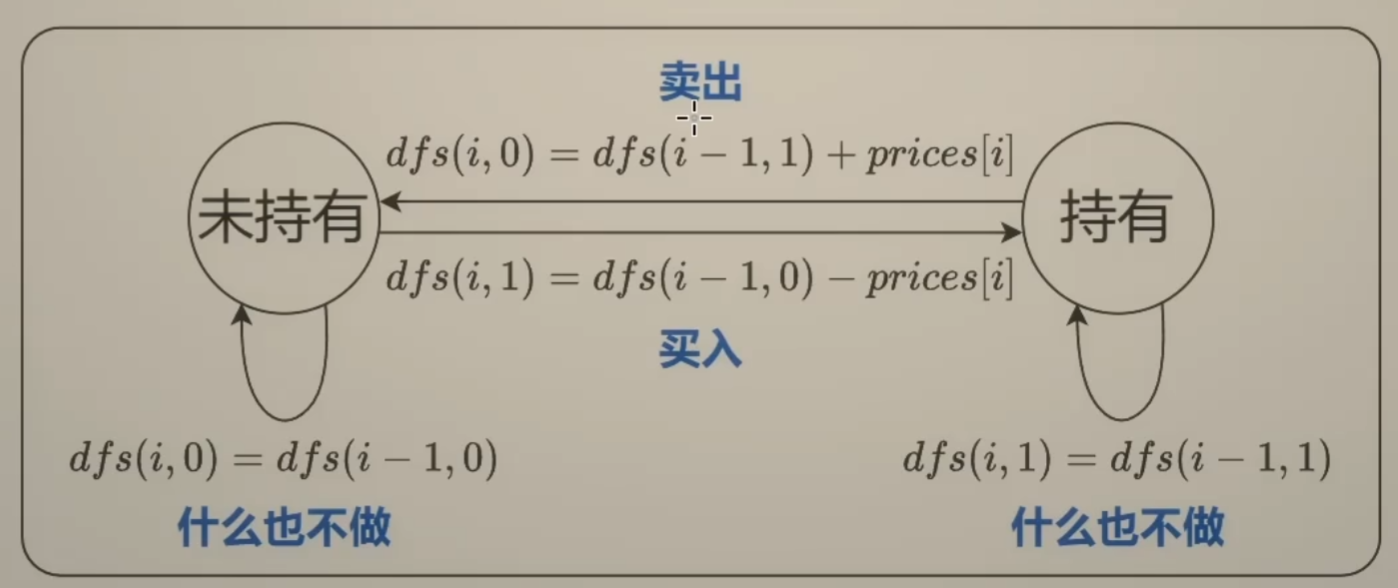
\includegraphics[width=0.8\textwidth]{state.png}
  \end{columns}
\end{frame}



\begin{frame}[fragile]          % 注意添加 fragile 标记
  \frametitle{\textsc{122. 买卖股票的最佳时机 II}\link{https://leetcode.cn/problems/best-time-to-buy-and-sell-stock-ii}}
  % 代码块参数:语言,标题
  % 请减少代码初始的缩进
  \begin{itemize}
    \item 我们每走到一个$i$,都会有两种状态$state$:持有$hold$股票,不持有$not \text{ } hold$股票。这就是我们用$1$代表持有,$0$代表未持有的思想了
    \item 到了$dp(i,1)$也就是第$i$时刻持有股票,有两种可能:
          \begin{itemize}
            \item 什么也不做,$dp(i,1)=dp(i-1,1)$
            \item $not\text{ } hold \to hold$,也就是$dp(i,1)=dp(i-1,0)-prices[i]$,因为我们持有了,买入股票了,手上的钱少了$prices[i]$,自然是$-$
            \item 合起来,就是$dp(i,1)=\max(dp(i-1,1),dp(i-1,0)-prices[i])$
          \end{itemize}
    \item 到了$dp(i,0)$也就是第$i$时刻\textbf{不}持有股票,有两种可能:
          \begin{itemize}
            \item 什么也不做,$dp(i,0)=dp(i-1,0)$
            \item $hold \to not\text{ } hold$,也就是$dp(i,0)=dp(i-1,1)+prices[i]$,因为我们卖股票了,不持有了,手上的钱多了$prices[i]$,自然是$+$
            \item 合起来,就是$dp(i,0)=\max(dp(i-1,0),dp(i-1,1)+prices[i])$
          \end{itemize}
    \item 最后一刻我们一定是希望手上股票全部卖出了,自然是对应了$not\text{ }hold$这个状态,\lstinline{return dp(n-1,0)}。特别的边界条件也就是我们什么股票都没得选\lstinline{if i < 0},如果没股票选还$hold$,那么必然不合理,自然就是$-\infty$。不持有自然就是$0$
  \end{itemize}
\end{frame}


\begin{frame}[fragile]
  \begin{codeblock}[language=python]{上手写代码吧,状态机\textsc{DP}最好画画状态转移图明确}
class Solution:
    def maxProfit(self, prices: List[int]) -> int:
        n = len(prices)
        @cache
        def dfs(i: int, hold: bool) -> int:
            if i < 0:
                return -inf if hold else 0
            if hold:
                return max(dfs(i - 1, False) - prices[i], dfs(i - 1, True))
            else:
                return max(dfs(i - 1, True) + prices[i], dfs(i - 1, False))
        return dfs(n - 1, False)
  \end{codeblock}
\end{frame}



\begin{frame}[fragile]
  \frametitle{1:1翻译成递推}
  \begin{codeblock}[language=python]{1:1翻译成递推}
class Solution:
    def maxProfit(self, prices: List[int]) -> int:
        n = len(prices)
        dp = [[0] * 2 for _ in range(n + 1)]
        dp[0][1] = -inf
        for i, p in enumerate(prices):
            dp[i + 1][1] = max(dp[i][1], dp[i][0] - p)
            dp[i + 1][0] = max(dp[i][0], dp[i][1] + p)
        return dp[n][0]
  \end{codeblock}
\end{frame}

\begin{frame}[fragile]
  \frametitle{1:1翻译成优化掉一个维度的递推}
  \begin{codeblock}[language=python]{优化掉这个二维的空间成一维空间}
class Solution:
    def maxProfit(self, prices: List[int]) -> int:
        dp0, dp1 = 0, -inf
        for p in prices:
            dp0, dp1 = max(dp0, dp1 + p), max(dp1, dp0 - p)
        return dp0
  \end{codeblock}
\end{frame}


\begin{frame}[fragile]          % 注意添加 fragile 标记
  \frametitle{\textsc{123. 买卖股票的最佳时机 III}\link{https://leetcode.cn/problems/best-time-to-buy-and-sell-stock-iii}}
  % 代码块参数:语言,标题
  % 请减少代码初始的缩进
    \begin{alertblock}{状态转移方程}
    % Taken from Mathmode.tex
    \begin{align}
      &dp(i,0,remaining)=\max(dp(i-1,0,remaining),dp(i-1,1,remaining-1)+price[i])\\
      &dp(i,1,remaining)=\max(dp(i-1,1,remaining),dp(i-1,0,remaining)-price[i])
    \end{align}
  \end{alertblock}
  \begin{itemize}
    \item 限制两次了,怎么思考呢?
    \item 一开始我们加了一个$hold$这个维度,那么既然限制两次,我们就加一个剩余$remaining$多少次可以交易的维度。那么就是$dp(i,hold,remaining)$。既然买卖是让$remaining-1$,那么我们“卖”,也就是$hold \to not\text{ } hold\implies remaining-1$,相反的“买”就没必要$remaining-1$了
    \item 边界条件:在前面的基础上,如果$remaining<0$,显然不合理,自然$-\infty$
  \end{itemize}
\end{frame}


\begin{frame}[fragile]
  \begin{codeblock}[language=python]{上手写记忆化搜索的代码吧}
class Solution:
    def maxProfit(self, prices: List[int]) -> int:
        @cache
        def dfs(i: int, hold: bool, remaining: int) -> int:
            if remaining < 0:
                return -inf
            if i < 0:
                return 0 if not hold else -inf
            if hold:
                return max(dfs(i - 1, True, remaining), dfs(i - 1, False, remaining) - prices[i])
            else:
                return max(dfs(i - 1, False, remaining), dfs(i - 1, True, remaining - 1) + prices[i])
        return dfs(len(prices) - 1, False, 2)
  \end{codeblock}
\end{frame}

\begin{frame}[fragile]
  \frametitle{1:1翻译成递推}
  \begin{codeblock}[language=python]{1:1翻译成递推}
class Solution:
    def maxProfit(self, prices: List[int]) -> int:
        k = 2
        f = [[-inf] * 2 for _ in range(k + 2)]
        for j in range(1, k + 2):
            f[j][0] = 0
        for p in prices:
            for j in range(k + 1, 0, -1):
                f[j][0] = max(f[j][0], f[j][1] + p)
                f[j][1] = max(f[j][1], f[j - 1][0] - p)
        return f[-1][0]
  \end{codeblock}
\end{frame}


\begin{frame}[fragile]          % 注意添加 fragile 标记
  \frametitle{\textsc{188. 买卖股票的最佳时机 IV}\link{https://leetcode.cn/problems/best-time-to-buy-and-sell-stock-iv}}
  % 代码块参数:语言,标题
  % 请减少代码初始的缩进
    \begin{alertblock}{状态转移方程}
    % Taken from Mathmode.tex
    \begin{align}
      &dp(i,0,remaining)=\max(dp(i-1,0,remaining),dp(i-1,1,remaining-1)+price[i])\\
      &dp(i,1,remaining)=\max(dp(i-1,1,remaining),dp(i-1,0,remaining)-price[i])
    \end{align}
  \end{alertblock}
  \begin{itemize}
    \item 跟上一题其实是一样的,无非是上一题$k=2$,不说了
  \end{itemize}
\end{frame}


\begin{frame}[fragile]
  \begin{codeblock}[language=python]{ }
class Solution:
    def maxProfit(self, k: int, prices: List[int]) -> int:
        @cache
        def dfs(i: int, hold: bool, remaining: int) -> int:
            if remaining < 0:
                return -inf
            if i < 0:
                return -inf if hold else 0
            res = -inf
            if hold:
                res = max(dfs(i - 1, False, remaining) - prices[i], dfs(i - 1, True, remaining))
            else:
                res = max(dfs(i - 1, False, remaining), dfs(i - 1, True, remaining - 1) + prices[i])
            return res
        res = dfs(len(prices) - 1, False, k)
        return res
  \end{codeblock}
\end{frame}


\begin{frame}[fragile]          % 注意添加 fragile 标记
  \frametitle{\textsc{309. 买卖股票的最佳时机含冷冻期}\link{https://leetcode.cn/problems/best-time-to-buy-and-sell-stock-with-cooldown}}
  % 代码块参数:语言,标题
  % 请减少代码初始的缩进
    \begin{alertblock}{状态转移方程}
    % Taken from Mathmode.tex
    \begin{align}
      &dp(i,0)=\max(dp(i-1,0),dp(i-1,1)+price[i])\\
      &dp(i,1)=\max(dp(i-1,1),dp(i-2,0)-price[i])
    \end{align}
  \end{alertblock}
  \begin{itemize}
    \item 冷冻期的意思是,我们第$i$天想买入$not \text{ } hold \to hold$,那么我们不可以从$dp(i-1,0)\to dp(i,1)$,而是$dp(i-2,0)\to dp(i,1)$递推,也就是隔一天
    \item 根据前面的推导,我们直接把$dp(i,1)=\max(dp(i-1,1),dp(i-1,0)-prices[i])$改成$dp(i,1)=\max(dp(i-1,1),dp(i-2,0)-prices[i])$就可以了
  \end{itemize}
\end{frame}


\begin{frame}[fragile]
  \frametitle{代码改起来相当容易}
  \begin{codeblock}[language=python]{记忆化搜索的代码}
class Solution:
    def maxProfit(self, prices: List[int]) -> int:
        n = len(prices)
        @cache
        def dfs(i: int, hold: bool) -> int:
            if i < 0:
                return 0 if not hold else -inf
            if hold:
                return max(dfs(i - 1, True), dfs(i - 2, False) - prices[i])
            else:
                return max(dfs(i - 1, False), dfs(i - 1, True) + prices[i])
        return dfs(n - 1, False)
  \end{codeblock}
\end{frame}


\begin{frame}[fragile]          % 注意添加 fragile 标记
  \frametitle{\textsc{714. 买卖股票的最佳时机含手续费}\link{https://leetcode.cn/problems/best-time-to-buy-and-sell-stock-with-transaction-fee}}
  % 代码块参数:语言,标题
  % 请减少代码初始的缩进
    \begin{alertblock}{状态转移方程}
    % Taken from Mathmode.tex
    \begin{align}
      &dp(i,0)=\max(dp(i-1,0),dp(i-1,1)+price[i]-fee)\\
      &dp(i,1)=\max(dp(i-1,1),dp(i-1,0)-price[i])
    \end{align}
  \end{alertblock}
  \begin{itemize}
    \item 有手续费无非是我们每次交易,不妨定义买$\to$卖是一次完整的交易,那么$hold \to not \text{ } hold$是一次交易结束,此时扣手续费$-fee$
    \item 那么无非就是把$dp(i-1,1)\to dp(i,0)$状态转移方程改改就行了。$dp(i,0)=\max(dp(i-1,0),dp(i-1,1)+price[i]-fee)$
  \end{itemize}
\end{frame}


\begin{frame}[fragile]
  \frametitle{代码改起来也很容易}
  \begin{codeblock}[language=python]{记忆化搜索的代码}
class Solution:
    def maxProfit(self, prices: List[int], fee: int) -> int:
        n = len(prices)
        @cache
        def dfs(i: int, hold: bool) -> int:
            if i < 0:
                return 0 if not hold else -inf
            if hold:
                return max(dfs(i - 1, True), dfs(i - 1, False) - prices[i])
            else:
                return max(dfs(i - 1, False), dfs(i - 1, True) + prices[i] - fee)
        return dfs(n - 1, False)
  \end{codeblock}
\end{frame}



\begin{frame}[fragile]          % 注意添加 fragile 标记
  \frametitle{至此我们的买卖股票的最佳时机专题已经讲完了}
  % 代码块参数:语言,标题
  % 请减少代码初始的缩进
  \begin{itemize}
    \item 我们概括一下状态机\textsc{DP}的核心
    \item 状态机\textsc{DP}的核心就是:$f[i][j]$表示前缀$a[:i]$在状态$j$下的最优值。$j$一般很小。这就是状态机\textsc{DP}怎么状态转移的
  \end{itemize}
\end{frame}


\begin{frame}[fragile]          % 注意添加 fragile 标记
  \frametitle{\textsc{3259. 超级饮料的最大强化能量}\link{https://leetcode.cn/problems/maximum-energy-boost-from-two-drinks}}
  % 代码块参数:语言,标题
  % 请减少代码初始的缩进
    \begin{alertblock}{状态转移方程}
    % Taken from Mathmode.tex
    \begin{align}
      &f(i,drinkA)=\max(f(i-1,drinkA),f(i-2,drinkB)+energyDrinkA[i])\\
      &f(i,drinkB)=\max(f(i-1,drinkB),f(i-2,drinkA)+energyDrinkB[i])
    \end{align}
  \end{alertblock}
  \begin{itemize}
    \item 这道题就是买卖股票和打家劫舍的变式。我们两个状态:到了第$i$个我们要么买$A$饮料要么买$B$饮料。我们用$f(i,j)$表示到了第$i$个,买$j$饮料,能量的最大值
    \item 如果我们想买$A$饮料获得能量最大,那么我们要么从$B$转向买$A$,要么不买,继承之前买的$A$获得的最大值。写成公式就是$f(i-1,drinkA)$,$f(i-2,drinkB)+energyDrinkA[i]$,因为我们也是要么买$A$,要么不买
    \item 同样的道理,我们也可以写出第二个状态的转移方程
    \item 边界条件我们什么都没买$i < 0$就必然获得$0$个能量了
  \end{itemize}
\end{frame}

\begin{frame}[fragile]
  \frametitle{就写一下记忆化搜索的代码吧,思路挺清晰的}
  \begin{codeblock}[language=python]{}
class Solution:
    def maxEnergyBoost(self, energyDrinkA: List[int], energyDrinkB: List[int]) -> int:
        n = len(energyDrinkA)
        @cache
        def dfs(i: int, drinkA: bool) -> int:
            if i < 0:
                return 0
            if drinkA:
                return max(dfs(i - 1, True), dfs(i - 2, False)) + energyDrinkA[i]
            else:
                return max(dfs(i - 1, False), dfs(i - 2, True)) + energyDrinkB[i]
        return max(dfs(n - 1, True), dfs(n - 1, False))
  \end{codeblock}
\end{frame}

\begin{frame}[fragile]          % 注意添加 fragile 标记
  \frametitle{\textsc{2826. 将三个组排序}\link{https://leetcode.cn/problems/sorting-three-groups}}
  % 代码块参数:语言,标题
  % 请减少代码初始的缩进
  %   \begin{alertblock}{}
  %   % Taken from Mathmode.tex
  %   \begin{align}
  %     &dp(i,0)=\max(dp(i-1,0),dp(i-1,1)+price[i]-fee)\\
  %     &dp(i,1)=\max(dp(i-1,1),dp(i-1,0)-price[i])
  %   \end{align}
  % \end{alertblock}
  \begin{itemize}
    \item 我们这么思考:删除了$nums$的一些数后,留下的一定是\textbf{非递减子序列}。那么我们记这个长度为$l$,那么我们删除的数一共有$len(nums)-l$,我们希望这个最小,那么一定是$l$最大
    \item 问题就是求$nums$的\textbf{最长递增子序列长度}了,经典$LIS$问题。这个题无非要求\textbf{最长非递减子序列问题}而已
  \end{itemize}
\end{frame}


\begin{frame}[fragile]
  \frametitle{没学过\textsc{LIS}问题的xdm就看看我怎么写的吧}
  \begin{codeblock}[language=python]{不需要按照李国强老师的\textsc{slides}写那个时间复杂度是$\mathcal{O}(n^2)$}
class Solution:
    def minimumOperations(self, nums: List[int]) -> int:
        def LIS(nums: List[int]) -> int:
            dp = []
            for num in nums:
                if not dp or num >= dp[-1]:
                    dp.append(num)
                else:
                    i = bisect_right(dp, num)
                    dp[i] = num
            return len(dp)
        return len(nums) - LIS(nums)
  \end{codeblock}
\end{frame}


\begin{frame}[fragile]          % 注意添加 fragile 标记
  \frametitle{这道题怎么用状态机\textsc{DP}来思考呢?}
  \begin{itemize}
    \item 我们这么想:我们记$f(i,j)$是到了$i$把$nums[0]\sim nums[i]$修改成\textbf{非递减子序列}的最小修改次数,而且此时以$j$结尾。毕竟$j$只可能取$1,2,3$
    \item 那么我们有了$dp[i][j]=\min\limits_{1\leq k \leq j}(1+dp[i-1][j])\text{ } if\text{ }j \neq nums[i]$,我们改了嘛自然修改次数$+1$
    \item $j == nums[i]$,那不用$+1$了毕竟不用修改
    \item 合起来就是$dp[i][j]=\min\limits_{1\leq k \leq j}(dp[i-1][j])\text{ } + (j\neq nums[i])$
  \end{itemize}
\end{frame}


\begin{frame}[fragile]
  \frametitle{写成优化一个维度的\textsc{DP}吧}
  \begin{codeblock}[language=python]{1:1翻译成递推}
class Solution:
    def minimumOperations(self, nums: List[int]) -> int:
        f = [0] * 4
        for x in nums:
            for j in range(3, 0, -1):
                f[j] = min(f[k] for k in range(1, j + 1)) + (j != x)
        return min(f[1:])
  \end{codeblock}
\end{frame}


\begin{frame}[fragile]{\LaTeX{} 常用环境}
  \begin{block}{环境}
    \centering
    \footnotesize
    \begin{tabular}{lll}
      \env{table}   & \env{figure}    & \env{equation}    \\
      表格            & 图片              & 公式                \\\hline
      \env{itemize} & \env{enumerate} & \env{description} \\
      无编号列表         & 编号列表            & 描述                \\\hline
    \end{tabular}
  \end{block}
\end{frame}
%
\begin{frame}{\LaTeX{}命令举例}
  \cmdxmp{chapter}{前言}{\heiti 第 1 章\hspace{1em} 前言}
  \cmdxmp{section[精简标题]}{这个题目实在太长了放到目录里面不太好看}{\heiti 1.1
    \hspace{1em} 这个题目实在太长了放到目录里面不太好看}
  \cmdxmp{footnote}{我是可爱的脚注}{前方高能\footnote{我是可爱的脚注}}
\end{frame}

\begin{frame}[fragile]{\LaTeX{} 环境举例}
  \begin{minipage}{0.4\linewidth}
    \begin{lstlisting}[basicstyle=\ttfamily\small]
\begin{itemize}
  \item 一条
  \item 次条
  \item 这一条可以分为 ...
    \begin{itemize}
      \item 子一条
    \end{itemize}
\end{itemize}
\end{lstlisting}
  \end{minipage}\hspace{1.5cm}
  \begin{minipage}{0.4\linewidth}
    \begin{itemize}
      \item 一条
      \item 次条
      \item 这一条可以分为 ...
            \begin{itemize}
              \item 子一条
            \end{itemize}
    \end{itemize}
  \end{minipage}
  \medskip

  \begin{minipage}{0.4\linewidth}
    \begin{lstlisting}
\begin{enumerate}
  \item 一条
  \item 次条
  \item 再条
\end{enumerate}
\end{lstlisting}
  \end{minipage}\hspace{1.5cm}
  \begin{minipage}{0.4\linewidth}
    \begin{enumerate}
      \item 一条
      \item 次条
      \item 再条
    \end{enumerate}
  \end{minipage}
\end{frame}
%

\begin{frame}[fragile]{\LaTeX{} 数学公式}

  \begin{columns}
    \begin{column}{.5\textwidth}
      \begin{lstlisting}[basicstyle=\ttfamily\small]
$V = \frac{4}{3}\pi r^3$

\[
  V = \frac{4}{3}\pi r^3
\]

\begin{equation}
\label{eq:vsphere}
V = \frac{4}{3}\pi r^3
\end{equation}
\end{lstlisting}
    \end{column}

    \begin{column}{.5\textwidth}
      $f[i][j]=\min\limits_{s \subseteq j}\max(f[i-1][j\setminus s],sum[s])$

      \[
        V = \frac{4}{3}\pi r^3
      \]

      \begin{equation}
        \label{eq:vsphere}
        V = \frac{4}{3}\pi r^3
      \end{equation}
    \end{column}
  \end{columns}

\end{frame}

\begin{frame}[fragile]{\LaTeX{} 数学公式}
  \begin{itemize}
    \item 数学公式排版是 \LaTeX{} 的绝对强项
    \item 数学排版需要进入数学模式,引用 \texttt{amsmath} 宏包
          \begin{itemize}
            \item 用单个美元符号(\verb|$|) 包围起来的内容是 {\bf 行内公式}
            \item 用两个美元符号(\verb|$$|) (不推荐)或
                  \verb|\[ \]| 包围起来的是 {\bf 单行公式} 或 {\bf 行间公式}
            \item 使用数学环境,例如 \texttt{equation} 环境内的公式会自动加上编号,
                  \texttt{align} 环境用于多行公式(例如方程组、多个并列条件等)
          \end{itemize}
    \item 寻找符号
          \begin{itemize}
            \item 运行 \texttt{texdoc symbols} 查看符号表
            \item S. Pakin. \emph{The Comprehensive \LaTeX{} Symbol List}
                  \link{https://ctan.org/pkg/comprehensive}
            \item 手写识别(有趣但不全):Detexify \link{http://detexify.kirelabs.org}
          \end{itemize}
    \item MathType 也可以使用和导出 \LaTeX{} 公式(不推荐)
  \end{itemize}
\end{frame}

%% 需要在导言区使用 \usepackage{unicode-math}
%
% \begin{frame}[fragile,label={frame:unicode-math}]{unicode-math:现代的数学输入方式}
%   \LaTeX{} 的公式确实很强大,但是……符号有点难记?

%   \pkg{unicode-math} 宏包提供了几乎所见即所得的公式输入:

%   \begin{itemize}
%     \item 可直接输入各类符号对应的 Unicode 字符(需要使用 UTF-8 编码):

%           \begin{columns}[c]
%             \begin{column}{0.45\textwidth}
%               \begin{lstlisting}
% \begin{equation*}
% ∫ Γ(x) dx = ±∞
% \end{equation*}
%       \end{lstlisting}
%             \end{column}\hspace{1em}
%             \begin{column}{0.45\textwidth}
%               \begin{equation*}
%                 ∫ Γ(x) dx = ±∞
%               \end{equation*}
%             \end{column}
%           \end{columns}
%     \item 使用 \verb|symbf| 等命令自动处理字母的粗体、斜体等变体,不必引入额外宏包。
%   \end{itemize}

%   \begin{columns}[c]
%     \begin{column}{0.45\textwidth}
%       \begin{lstlisting}
% \begin{align*}
% \symbf{\beta} &= \beta \symbf{I} \\
% \symbf{a} &= a \symbf{I}
% \end{align*}
% \end{lstlisting}
%     \end{column}\hspace{1em}
%     \begin{column}{0.45\textwidth}
%       \begin{align*}
%         \symbf{\beta} & = \beta \symbf{I} \\
%         \symbf{a}     & = a \symbf{I}
%       \end{align*}
%     \end{column}
%   \end{columns}

% \end{frame}

\begin{frame}[fragile]{层次与目录生成}
  \begin{columns}
    \begin{column}{.6\textwidth}

      \begin{lstlisting}[basicstyle=\ttfamily\small,morekeywords={
        tableofcontents, part, chapter, section, subsection, subsubsection,
        paragraph, subparagraph}]
\tableofcontents % 这里是目录
\part{有监督学习}
\chapter{支持向量机}
\section{支持向量机简介}
\subsection{支持向量机的历史}
\subsubsection{支持向量机的诞生}
\paragraph{一些趣闻}
\subparagraph{第一个趣闻}
\end{lstlisting}
    \end{column}
    \begin{column}{.4\textwidth}
      第一部分\quad 有监督学习\\
      第一章\quad 支持向量机 \\
      1. 支持向量机简介 \\
      1.1 支持向量机的历史 \\
      1.1.1 支持向量机的诞生 \\
      一些趣闻  \\
      第一个趣闻
    \end{column}
  \end{columns}

\end{frame}

\begin{frame}[fragile]{列表与枚举}
  \begin{columns}
    \begin{column}{.6\textwidth}
      \begin{lstlisting}[basicstyle=\ttfamily\small]
\begin{enumerate}
\item \LaTeX{} 好处都有啥
  \begin{description}
    \item[好用] 体验好才是真的好
    \item[好看] 强迫症的福音
    \item[开源] 众人拾柴火焰高
  \end{description}
\item 还有呢?
  \begin{itemize}
    \item 好处 1
    \item 好处 2
  \end{itemize}
\end{enumerate}
\end{lstlisting}
    \end{column}
    \begin{column}{.4\textwidth}
      {\small
        \begin{enumerate}
          \item \LaTeX{} 好处都有啥
                \begin{description}
                  \item[好用] 体验好才是真的好
                  \item[好看] 治疗强迫症
                  \item[开源] 众人拾柴火焰高
                \end{description}
          \item 还有呢?
                \begin{itemize}
                  \item 好处 1
                  \item 好处 2
                \end{itemize}
        \end{enumerate}
      }
    \end{column}
  \end{columns}

\end{frame}

\begin{frame}[fragile]{交叉引用与插入插图}
  \begin{itemize}
    \item 给对象命名:图片、表格、公式等\\
          \verb|\label{name}|
    \item 引用对象\\
          \verb|\ref{name}|
  \end{itemize}
  \bigskip

  \begin{minipage}{0.7\linewidth}
    \begin{lstlisting}
交大校徽请参见图~\ref{fig:badge}。
\begin{figure}[htbp]
  \centering
  \includegraphics[height=.2\textheight]%
  {sjtu-badge-blue.pdf}
  \caption{交大校徽。}
  \label{fig:badge}
\end{figure}
\end{lstlisting}
  \end{minipage}\hfill
  \begin{minipage}{0.3\linewidth}\centering
    {\songti 交大校徽请参见图~1。}\\[1em]
    \includegraphics[height=0.2\textheight]{sjtu-badge-blue.pdf}\\
    {\footnotesize\heiti 图~1. 交大校徽。}
  \end{minipage}
\end{frame}

\begin{frame}[fragile]{交叉引用与插入表格}
  \vspace{-1.5em}
  \begin{columns}
    \column{.6\textwidth}
    \begin{lstlisting}
\begin{table}[htbp]
   \caption{编号与含义}
   \label{tab:number}
   \centering
   \begin{tabular}{cl}
     \toprule
     编号 & 含义 \\
     \midrule
     1    & 第一 \\
     2    & 第二 \\
     \bottomrule
   \end{tabular}
\end{table}
公式~(\ref{eq:vsphere}) 中编号与含义
请参见表~\ref{tab:number}。
\end{lstlisting}
    \column{.4\textwidth}
    \centering
    {\small 表~1. 编号与含义}\\[2pt]
    \begin{tabular}{cl}\toprule
      编号 & 含义 \\\midrule
      1  & 第一 \\
      2  & 第二 \\\bottomrule
    \end{tabular}\\[5pt]

    \normalsize 公式~(\ref{eq:vsphere})编号与含义请参见表~1。
  \end{columns}
\end{frame}

\begin{frame}[fragile]{浮动体}
  \begin{itemize}
    \item 初学者最“捉摸不透”的特性之一
          \link{https://liam.page/2017/03/11/floats-in-LaTeX-basic}
    \item 图片和表格有时会很大,在插入的位置不一定放得下,因此需要浮动调整
    \item 避免在文中使用「下图」「上图」的说法,而是使用图表的编号,例如 \verb|图~\ref{fig:fig1}| 。
    \item \verb|\begin{figure}[<位置>] 图片 \end{figure}|
          \begin{itemize}
            \item 位置参数指定浮动体摆放的偏好
            \item \verb|h| 当前位置(here), \verb|t|
                  顶部(top), \verb|b| 底部(bottom),
                  \verb|p| 单独成页(p)
            \item \verb|!h| 表示忽略一些限制,\verb|H|
                  表示强制\alert{(强烈不建议,除非你知道自己在做什么)}
          \end{itemize}
    \item 温馨提示:图标题一般在下方,表标题一般在上方
  \end{itemize}
\end{frame}

\begin{frame}[fragile]
  \frametitle{作图与插图}
  \begin{itemize}
    \item 外部插入

          \begin{itemize}
            \item Mathematica、MATLAB
            \item PowerPoint、Visio、Adobe Illustrator、Inkscape
            \item Python \pkg{Matplotlib} 库、\texttt{Plots.jl}、R、Plotly 等
            \item draw.io \link{https://draw.io/}、ProcessOn \link{https://www.processon.com/}
                  等在线绘图网站
          \end{itemize}

    \item \TeX{} 内联

          \begin{itemize}
            \item Asymptote
            \item \alert{\pkg{pgf}/\pkg{TikZ}、\pkg{pgfplots}}
          \end{itemize}

    \item 插图格式

          \begin{itemize}
            \item 矢量图:\verb|.pdf|
            \item 位图:\verb|.jpg| 或 \verb|.png|
            \item \alert{不再推荐 \texttt{.eps}}
            \item 不(完全)支持 \verb|.svg|、\verb|.bmp|
          \end{itemize}

    \item 一些参考:\link{https://www.zhihu.com/question/21664179}
          \link{https://tex.stackexchange.com/q/158668}
          \link{https://tex.stackexchange.com/q/72930}
  \end{itemize}
\end{frame}

\begin{frame}[fragile]{表格绘制}
  \begin{itemize}
    \item 使用 \pkg{booktabs}、\pkg{longtables}、\pkg{multirow} 等宏包
    \item 手动绘制表格确实比较令人头疼,且较难维护
    \item 推荐使用在线工具绘制后导出代码:\LaTeX{} Table Generator
          \link{https://www.tablesgenerator.com/latex_tables}
  \end{itemize}
\end{frame}

\begin{frame}[fragile]{文献引用}
  \begin{itemize}
    \item 新时期我国信息技术产业的发展 \cite{devoftech}
    \item 他改变了中国 \cite{thelegendofjiang}
  \end{itemize}
\end{frame}

\begin{frame}[fragile]
  \frametitle{宏包推荐(先读文档后使用)}
  \vspace{-1.5em}
  \scriptsize
  \begin{multicols}{3}
    \begin{itemize}
      \item 必备

            \begin{itemize}
              \item \pkg{amsmath}
              \item \pkg{graphicx}
              \item \pkg{hyperref}
            \end{itemize}

      \item 样式

            \begin{itemize}
              \item \pkg{caption}
              \item \pkg{enumitem}
              \item \pkg{fancyhdr}
              \item \pkg{footmisc}
              \item \pkg{geometry}
              \item \pkg{titlesec}
            \end{itemize}

      \item 数学

            \begin{itemize}
              \item \pkg{bm}
              \item \pkg{mathtools}
              \item \pkg{physics}
              \item \pkg{unicode-math}
            \end{itemize}

      \item 表格

            \begin{itemize}
              \item \pkg{array}
              \item \pkg{booktabs}
              \item \pkg{longtable}
              \item \pkg{tabularx}
            \end{itemize}

      \item 插图、绘图

            \begin{itemize}
              \item \pkg{float}
              \item \pkg{pdfpages}
              \item \pkg{standalone}
              \item \pkg{subfigure}
              \item \pkg{pgf}/\pkg{tikz}
              \item \pkg{pgfplots}
            \end{itemize}

      \item 字体

            \begin{itemize}
              \item \pkg{newpx}
              \item \pkg{pifont}
              \item \pkg{fontspec}
            \end{itemize}

      \item 各种功能

            \begin{itemize}
              \item \pkg{algorithm2e}
              \item \pkg{beamer}
              \item \pkg{biblatex}
              \item \pkg{listings}
              \item \pkg{mhchem}
              \item \pkg{microtype}
              \item \pkg{minted}
              \item \pkg{natbib}
              \item \pkg{siunitx}
              \item \pkg{xcolor}
            \end{itemize}

      \item 多语言

            \begin{itemize}
              \item \pkg{babel}
              \item \pkg{polyglossia}
              \item \pkg{ctex}
              \item \pkg{xeCJK}
            \end{itemize}
    \end{itemize}
  \end{multicols}
  \vspace*{-0.5cm}
\end{frame}

\subsection{论文模板使用}

\begin{frame}{模板是什么?}
  \begin{itemize}
    \item 模板
          \begin{itemize}
            \item 已经设计好的格式框架
            \item 好的模板:使用户专注于内容
            \item 不应将时间花费在调整框架上
          \end{itemize}
    \item 再提 Office 和 Word
          \begin{itemize}
            \item 很少有人会有意识地在 Word 中使用模板
            \item 定义自己的标题?定义自己的列表?定义自己的段落样式?
            \item 自动化,还是手工调?
            \item 经常被折腾的精疲力竭
            \item 学习 \LaTeX{} 能帮助自己更好科学地使用 Word
          \end{itemize}
  \end{itemize}
\end{frame}

\begin{frame}{论文排版}
  \begin{itemize}
    \item 获取模板
          \begin{itemize}
            \item 随发行版自带、手动网络下载
            \item 模板文档类 \texttt{.cls} 文件
            \item 示例 \texttt{.tex} 文件
          \end{itemize}
    \item 编辑 \texttt{.tex} 文件:添加用户内容
    \item 编译:生成 PDF 文档
  \end{itemize}
\end{frame}

\begin{frame}[fragile]{论文排版举例}
  \begin{block}{IEEE 期刊论文}
    \begin{itemize}
      \item 获取模板:已随发行版自带
            \begin{itemize}
              \item 在安装目录 \verb|<prefix>/texlive/2023/texmf-dist/doc/latex/IEEEtran|
                    下找到 \verb|bare_jrnl.tex|
              \item 复制到某个文件夹(比如个人存论文的目录)
            \end{itemize}
      \item 编辑 \verb|bare_jrnl.tex| 文件 (英文模板:不支持中文)
      \item 编译
            \begin{itemize}
              \item 英文文献:\XeLaTeX{}、\pdfLaTeX{} 编译均可
            \end{itemize}
    \end{itemize}
  \end{block}
\end{frame}
